%% статьи в формате LaTeX для сборника статей "Системное         **
%% **  программирование".                                                   **
%% **  СПбГУ, мат.-мех. факультет, НИИ ИТ, 2005 г.                          **
%% **  Текст собирается с помощью программы latex                           **
%% **                                                                       **
%% ***************************************************************************

\documentclass[a5paper]{article}
\usepackage[a5paper, top=17mm, bottom=17mm, left=17mm, right=17mm]{geometry}
\usepackage[T2A]{fontenc} 
\usepackage[utf8]{inputenc}
\usepackage[english,russian]{babel}
\usepackage{graphicx}
\usepackage{indentfirst}
\usepackage{hyperref}
\usepackage{textcomp}


\sloppy
\pagestyle{empty}

%% ***************************************************************************
%% **                                                                       **
%% **  Место для названия статьи                                            **
%% **                                                                       **
%% ***************************************************************************
\title{Синтаксический анализ регулярных множеств}

%% ***************************************************************************
%% **                                                                       **
%% **  Место для авторов, их email-адресов и названий институтов            **
%% **                                                                       **
%% ***************************************************************************
%\author{С.В.Григорьев\\
%rsdpisuy@gmail.com\\
%\and Санкт-Петербургский государственный университет\\
%198504, Университетский проспект, 28, Старый Петергоф,\\
%Санкт-Петербург, Россия}
%\date{}
\begin{document}

%\maketitle
%\thispagestyle{empty}

%% ***************************************************************************
%% **                                                                       **
%% ** Аннотация                                                             **
%% **                                                                       **
%% ***************************************************************************
%\begin{quote}

%\renewcommand{\thefootnote}{}

%% ***************************************************************************
%% **                                                                       **
%% ** Авторские права                                                       **
%% **                                                                       **
%% ***************************************************************************
%\setcounter{footnote}{0}
%\end{quote}

%% ***************************************************************************
%% **                                                                       **
%% ** Текст статьи                                                          **
%% **                                                                       **
%% ***************************************************************************
\section{Немного про грамматики}

Предполагаемую структуру свёртки можно описать КС-грамматикой. При этом можно использовать более 
выразительные конструкции, чем нормальная форма Хомского (НФХ). В результате можно пытаться описать 
именно вторичную структуру, а не содержимое конкретной цепочки. При этом возможно как уточнение 
содержимого, так и ослабление структуры.

Конструкции, расширяющие НФХ, доступные для описания вторичной структуры. 
\begin{itemize}
    \item \textbf{Регулярные выражения}. Доступны операции $\{+,*,|,?\}$. Например, любой из символов 
    $\{A,U,G,C\}$, повторённый не менее 1 раза.
        \begin{verbatim}
    any : (A | U | G | C)+ 
        \end{verbatim}
    \item \textbf{Повторения} позволяют ограничивать количество однотипных элементов (в отличии от +*). Например, повторение \texttt{any} от 2 до 5 раз включительно:
        \begin{verbatim}
    s : any*[2..5] 
        \end{verbatim}
    \item \textbf{Метаправила} позволяют описывать параметризуемые шаблоны вывода. Например, шаблон 
вывода списка, пареметризованный элементом списка и разделителем.
        \begin{verbatim}
    not_empty_list<item sep>: item (sep item)*
        \end{verbatim}
    Применение описанного выше шаблона. Фактическими аргументами метаправила могут быть 
    произвольные конструкции: регулярные выражения, другие метаправила.
        \begin{verbatim}
    s1: not_empty_list<NUM COLON>
    s2: not_empty_list<s1 (DOT|COMMA)>
        \end{verbatim}
\end{itemize}

Возможный пример описания свёртки для tRNA.

\begin{verbatim}
[<Start>]
folded: stem<(any*[1..3] 
              stem<any*[4..10]> 
              any*[1..3] 
              stem<any*[4..7]> 
              any*[3..5] 
              stem<any*[4..7]>
              )>

stem<s>: 
      A stem<s> U
    | U stem<s> A
    | C stem<s> G
    | G stem<s> C
    | G stem<s> U
    | U stem<s> G
    | s

any: A | U | G | C

\end{verbatim}

Можно добавить вероятности для фильтрации деревьев. Применимы те же фильтры, что и в работах на 
основе CYK.

\begin{verbatim}
[<Start>]
folded: stem<(any*[1..3] 
              stem<any*[4..10]> 
              any*[1..3] 
              stem<any*[4..7]> 
              any*[3..5] 
              stem<any*[4..7]>
              )>

stem<s>: 
      [p1] (A stem<s> U)
    | [p1] (U stem<s> A)
    | [p1] (C stem<s> G)
    | [p1] (G stem<s> C)
    | [p2] (G stem<s> U)
    | [p2] (U stem<s> G)
    | [p3] (s)

a1: [p1] (A)
  | [p1] (U)
  | [p1] (G)
  | [p1] (C)
\end{verbatim}

Грамматика может быть модульной. Это позволяет описать некоторые базовые элементы отдельно и далее 
использовать, подключая соответствующие модули/модуль. Например, в переиспользуемый модуль можно 
вынести определение для \texttt{stem, any, R, Y} и другие элементы.

Опсле работы алгоритма доступны все деревья разбора, соответствующие хаданной грамматике, а значит 
и вторичной структуре. Далее, эти деревья сожно обрабатывать отдельно. Например, отбирать более 
вероятные используя различные фильтры, метрики, шаблоны. 

Что можно ещё интересного делать.
\begin{itemize} 
\item Пытаться восстанавливать грамматики из известных структур свёрток, а не описывать руками~\cite{SCFGRNA1}.
\item Восстановливать деревья по известным свёрткам.
\item Использовать структурные фильтры для деревьев.
\end{itemize}

\section{Технические детали}
Технически, задача достаточно хорошо масштабируемая. Возможно использование смешанных вычислений: CPU + GPGPU. В качестве алгоритма можно применять не только CYK, но и другие 
алгоритмы, которые могут оказаться более эффективными.

На Infernal я посмотрел. Внутри жуть что происходит. Код хоть и снабжён комментариями, но крайне плохо написан. Я не смог за 2 дня придумать, как быстро его передизайнить, чтобы он работал с графом, 
хотя для этого требуется просто другая раскладка матрицы, используемой в CYK. Что при аккуратном 
дизайне не должно вызывать проблем.


%\begin{figure}
%    \begin{center}
%        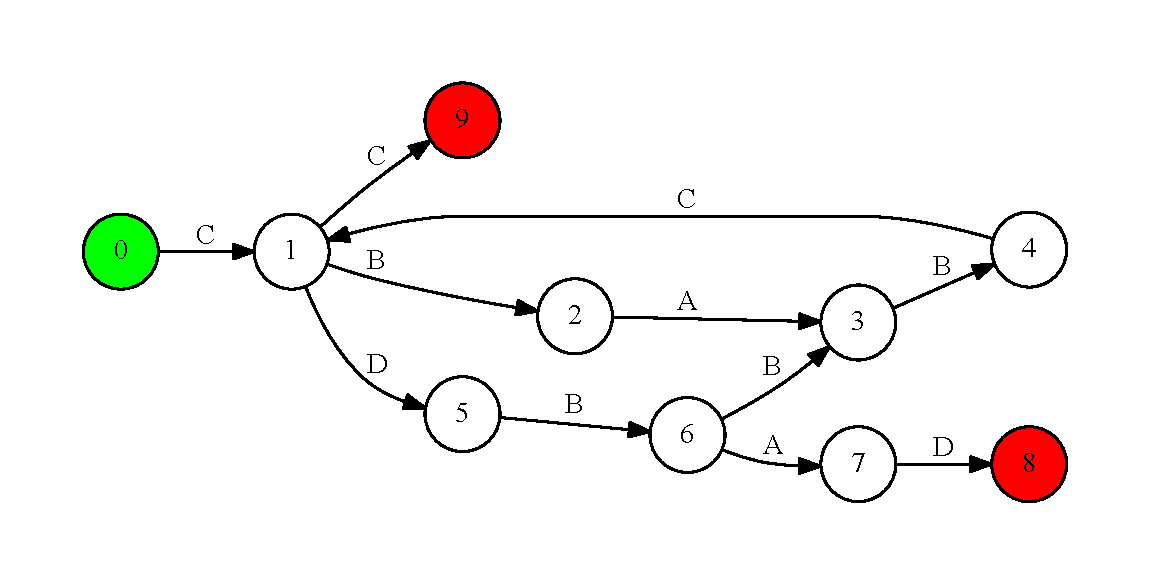
\includegraphics[width=11cm]{input.pdf}
%        \caption{Входной граф}
%        \label{pic1}        
%    \end{center}
%\end{figure}
%


%% ***************************************************************************
%% **                                                                       **
%% ** Список литературы                                                     **
%% **                                                                       **
%% ***************************************************************************
\begin{thebibliography}{99}
  
\bibitem{SCFGRNA1}
Dowell R. D., Eddy S. R. Evaluation of several lightweight stochastic context-free grammars for RNA 
secondary structure prediction //BMC bioinformatics. --- 2004. --- Т. 5. --- \textnumero. 1. --- С. 1.

\bibitem{SCFGRNA2}
Eddy S. R. A memory-efficient dynamic programming algorithm for optimal alignment of a sequence to 
an RNA secondary structure //BMC bioinformatics. --- 2002. --- Т. 3. --- \textnumero. 1. --- С. 1.
\end{thebibliography}

\end{document}
